% answers.tex —— 2007 年·普通高等学校招生考试·广东卷·文科 · 参考答案与详细解析片段
% 由 tools/generate_projects.py 依来源总账自 2007/2007_数学真题_广东文_试题.md + 2007/2007_数学真题_广东文_解析正文.md + 2007/2007_数学真题_广东文_答案要点.md 生成，勿手改（改源 MD 后重跑）


\begin{gktip}
固定候选 PDF 仅含题面，无答案、解析和评分标准，原卷亦未标注分值；以下为非官方编者独立推导，官方答案字段为空。来源发布者、出版者、版次与官方身份均未核。
\end{gktip}

\begin{answer}
\gksolhead{1}{}

\textbf{题目}：

已知集合 $M=\{x\mid 1+x>0\}$，$N=\left\{x\;\middle|\;\dfrac{1}{1-x}>0\right\}$，则 $M\cap N=$（　）

（A）$\{x\mid -1\leqslant x<1\}$

（B）$\{x\mid x>1\}$

（C）$\{x\mid -1<x<1\}$

（D）$\{x\mid x\geqslant -1\}$

\Needspace{4\baselineskip}
\textbf{解析}

\Needspace{5\baselineskip}
由 $1+x>0$ 得

\nopagebreak[4]
\[M=\{x\mid x>-1\}=(-1,+\infty).\]

\Needspace{5\baselineskip}
由 $\dfrac{1}{1-x}>0$ 知分母为正，即 $1-x>0$，得

\nopagebreak[4]
\[N=\{x\mid x<1\}=(-\infty,1).\]

\Needspace{5\baselineskip}
故

\nopagebreak[4]
\[M\cap N=(-1,1)=\{x\mid -1<x<1\},\]

选 C。

（判断要点：$\dfrac{1}{1-x}>0$ 等价于 $1-x>0$，不要误写成 $1-x\neq0$。）

\gkanswer{答案：C。}

\end{answer}
\begin{answer}
\gksolhead{2}{}

\textbf{题目}：

若复数 $(1+b\mathrm i)(2+\mathrm i)$ 是纯虚数（$\mathrm i$ 是虚数单位，$b$ 是实数），则 $b=$（　）

（A）$-2$

（B）$-\dfrac12$

（C）$\dfrac12$

（D）$2$

\Needspace{4\baselineskip}
\textbf{解析}

\Needspace{5\baselineskip}
展开复数：

\nopagebreak[4]
\[(1+b\mathrm i)(2+\mathrm i)=2+\mathrm i+2b\mathrm i+b\mathrm i^2=(2-b)+(1+2b)\mathrm i.\]

\Needspace{5\baselineskip}
纯虚数要求实部为零、虚部不为零：

\nopagebreak[4]
\[2-b=0\ \Rightarrow\ b=2,\]

此时虚部 $1+2b=5\neq0$，符合要求，选 D。

（判断要点：纯虚数必须同时满足实部为 $0$ 与虚部不为 $0$；只写 $2-b=0$ 而忘了检验虚部，会漏掉对 $b$ 的限制。）

\gkanswer{答案：D。}

\end{answer}
\begin{answer}
\gksolhead{3}{}

\textbf{题目}：

若函数 $f(x)=x^3$（$x\in\mathbf R$），则函数 $y=f(-x)$ 在其定义域上是（　）

（A）单调递减的偶函数

（B）单调递减的奇函数

（C）单调递增的偶函数

（D）单调递增的奇函数

\Needspace{4\baselineskip}
\textbf{解析}

\nopagebreak[4]
\[y=f(-x)=(-x)^3=-x^3.\]

其定义域为 $\mathbf R$，且 $(-x)^3=-x^3$ 关于原点对称，是奇函数；又 $y=-x^3$ 在 $\mathbf R$ 上单调递减，故选 B。

（判断要点：先求 $f(-x)$ 的解析式再判奇偶与单调，不要凭 $f(x)=x^3$ 的印象直接选“递增”。）

\gkanswer{答案：B。}

\end{answer}
\begin{answer}
\gksolhead{4}{}

\textbf{题目}：

若向量 $\boldsymbol a$，$\boldsymbol b$ 满足 $|\boldsymbol a|=|\boldsymbol b|=1$，$\boldsymbol a$ 与 $\boldsymbol b$ 的夹角为 $60^\circ$，则 $\boldsymbol a\cdot\boldsymbol a+\boldsymbol a\cdot\boldsymbol b=$（　）

（A）$\dfrac12$

（B）$\dfrac32$

（C）$1+\dfrac{\sqrt3}{2}$

（D）$2$

\Needspace{4\baselineskip}
\textbf{解析}

\Needspace{5\baselineskip}
由数量积定义，

\nopagebreak[4]
\[\boldsymbol a\cdot\boldsymbol a=|\boldsymbol a|^2=1,\qquad \boldsymbol a\cdot\boldsymbol b=|\boldsymbol a||\boldsymbol b|\cos60^\circ=\frac12.\]

\Needspace{5\baselineskip}
相加得

\nopagebreak[4]
\[\boldsymbol a\cdot\boldsymbol a+\boldsymbol a\cdot\boldsymbol b=1+\frac12=\frac32,\]

选 B。

（判断要点：夹角 $60^\circ$ 对应余弦 $\dfrac12$，两向量模都是 $1$，不要漏乘模长。）

\gkanswer{答案：B。}

\end{answer}
\begin{answer}
\gksolhead{5}{}

\textbf{题目}：

客车从甲地以 $60\ \mathrm{km/h}$ 的速度匀速行驶 $1$ 小时到达乙地，在乙地停留了半小时，然后以 $80\ \mathrm{km/h}$ 的速度匀速行驶 $1$ 小时到达丙地。下列描述客车从甲地出发，经过乙地，最后到达丙地所经过的路程 $s$ 与时间 $t$ 之间关系的图象中，正确的是（　）
\nopagebreak[4]
\begin{center}% 2007 年广东卷文科第 5 题：四个 s-t 图象选项（A）—（D）。
%   客车：0—1 h 以 60 km/h 行驶（s: 0→60），1—1.5 h 停留（s=60），
%   1.5—2.5 h 以 80 km/h 行驶（s: 60→140）。
%   （A）第二段升到 160；（B）无停留段且两段断开；（D）第二段斜率偏小；
%   （C）与解析式一致。
% 来源 PDF：gaokaomath-src/普通高考/2007/2007广东文.pdf
% SHA-256：6c8a7179f8b64b91f8f189f0aca7da3523d5d42dd5b8d2c8e9c0d3c6998459ee
% 原页：2007广东文.pdf 第 1 页（A3 三栏）第 1 栏，书页码 373，图在第 5 题题干下方。
% 重绘依据：按原页四个小图的折线顶点逐个比对；网格 0.25 h × 20 km，
%   横轴 0—3 h、纵轴 0—160 km，各图第二段斜率差异按原图保留。
\begin{tikzpicture}[x=1cm, y=0.032cm, semithick,
  every node/.style={inner sep=1.5pt}]

  % ---------------- 单个小图的公共网格 ----------------
  \newcommand{\stgrid}{%
    \foreach \gx in {0.25,0.5,...,3.0} {\draw[gray!45,very thin] (\gx,0) -- (\gx,160);}%
    \foreach \gy in {20,40,...,160} {\draw[gray!45,very thin] (0,\gy) -- (3.05,\gy);}%
    \draw[->,>=stealth] (0,0) -- (3.55,0) node[below right=1pt] {$t$ (h)};%
    \draw[->,>=stealth] (0,0) -- (0,178) node[left] {$s$ (km)};%
    \foreach \tx in {1,2,3} {\node[below] at (\tx,0) {$\tx$};}%
    \foreach \ty in {60,80,100,120,140,160} {\node[left] at (0,\ty) {$\ty$};}%
    \node[below left] at (0,0) {$O$};%
  }

  % ---------------- （A） ----------------
  \begin{scope}[shift={(0cm,0cm)}]
    \stgrid
    \draw[line width=1.1pt] (0,0) -- (1,60) -- (1.5,60) -- (2.5,160);
    \node at (1.7,-32) {（A）};
  \end{scope}

  % ---------------- （B） ----------------
  \begin{scope}[shift={(5.6cm,0cm)}]
    \stgrid
    \draw[line width=1.1pt] (0,0) -- (1,60);
    \draw[line width=1.1pt] (1.15,62) -- (2.6,140);
    \node at (1.7,-32) {（B）};
  \end{scope}

  % ---------------- （C） ----------------
  \begin{scope}[shift={(0cm,-7.2cm)}]
    \stgrid
    \draw[line width=1.1pt] (0,0) -- (1,60) -- (1.5,60) -- (2.5,140);
    \node at (1.7,-32) {（C）};
  \end{scope}

  % ---------------- （D） ----------------
  \begin{scope}[shift={(5.6cm,-7.2cm)}]
    \stgrid
    \draw[line width=1.1pt] (0,0) -- (1,60) -- (1.6,60) -- (2.8,140);
    \node at (1.7,-32) {（D）};
  \end{scope}
\end{tikzpicture}
\end{center}
\nopagebreak[4]
\Needspace{4\baselineskip}
\textbf{解析}

分三段写解析式：$0\leqslant t\leqslant1$ 时 $s=60t$；$1\leqslant t\leqslant1.5$ 时 $s=60$（停留）；$1.5\leqslant t\leqslant2.5$ 时 $s=60+80(t-1.5)$。图象特征是「先升、再平、再升」，且第二段斜率 $80$ 大于第一段斜率 $60$，终点 $(2.5,140)$。

对照选项：（A）第二段升到 $160$，斜率偏大；（B）两段之间断开且没有停留段；（D）第二段斜率偏小、终点时间偏晚；（C）三段折线与解析式一致，选 C。

（判断要点：停留半小时在图上是一段水平线，长度只占 $0.5$ 小时；先算出终点 $s=60+80=140$，可排除升到 $160$ 的选项。）

\gkanswer{答案：C。}

\end{answer}
\begin{answer}
\gksolhead{6}{}

\textbf{题目}：

若 $l$，$m$，$n$ 是互不相同的空间直线，$\alpha$，$\beta$ 是不重合的平面，则下列命题中为真命题的是（　）

（A）若 $\alpha\parallel\beta$，$l\subset\alpha$，$n\subset\beta$，则 $l\parallel n$

（B）若 $\alpha\perp\beta$，$l\subset\alpha$，则 $l\perp\beta$

（C）若 $l\perp n$，$m\perp n$，则 $l\parallel m$

（D）若 $l\perp\alpha$，$l\parallel\beta$，则 $\alpha\perp\beta$

\Needspace{4\baselineskip}
\textbf{解析}

逐项判断。

（A）$\alpha\parallel\beta$ 时，$l\subset\alpha$ 与 $n\subset\beta$ 可以异面，不一定平行，假。

（B）$\alpha\perp\beta$ 时，面 $\alpha$ 内只有垂直于交线的直线才垂直于 $\beta$，假。

（C）$l\perp n$，$m\perp n$ 时 $l$ 与 $m$ 可以相交、平行或异面，假。

（D）$l\perp\alpha$ 且 $l\parallel\beta$：$l$ 的方向是 $\alpha$ 的法向，而 $l$ 平行于 $\beta$ 说明 $l$ 的方向也在 $\beta$ 内（或与 $\beta$ 平行），于是 $\alpha$ 的法向落在 $\beta$ 内，$\alpha\perp\beta$，真。

选 D。

（判断要点：面面垂直的判定要找「一个平面过另一个平面的垂线」；（D）中 $l\parallel\beta$ 正是把 $l$ 平移到 $\beta$ 内的依据。）

\gkanswer{答案：D。}

\end{answer}
\begin{answer}
\gksolhead{7}{}

\textbf{题目}：

图 1 是某县参加 $2007$ 年高考的学生身高条形统计图，从左到右的各条形表示的学生人数依次记为 $A_1$，$A_2$，$\cdots$，$A_{10}$（如 $A_2$ 表示身高（单位：$\mathrm{cm}$）在 $[150,155)$ 内的学生人数）。图 2 是统计图 1 中身高在一定范围内学生人数的一个算法流程图。现要统计身高在 $160\sim180\ \mathrm{cm}$（含 $160\ \mathrm{cm}$，不含 $180\ \mathrm{cm}$）的学生人数，那么在流程图中的判断框内应填写的条件是（　）
\nopagebreak[4]
\begin{center}% 2007 年广东卷文科第 7 题：图 1 身高条形统计图。
%   十组 [145,150)—[190,195)，人数依次 A1—A10 =
%   100、200、320、450、550、500、360、220、80、40（按原页柱高读取）。
%   原点处纵轴刻度由 0 折断到 50，图下 0 为人数原点，横轴标签为各柱左右分界。
% 来源 PDF：gaokaomath-src/普通高考/2007/2007广东文.pdf
% SHA-256：6c8a7179f8b64b91f8f189f0aca7da3523d5d42dd5b8d2c8e9c0d3c6998459ee
% 原页：2007广东文.pdf 第 1 页（A3 三栏）第 2 栏，书页码 373。
% 重绘依据：横轴每格 5 cm、纵轴每格 50 人；0 与 50 之间按原图加折断线。
\begin{tikzpicture}[x=0.75cm, y=0.0085cm, semithick,
  every node/.style={inner sep=1.5pt, font=\small}]

  % 纵轴网格与刻度
  \foreach \gy in {50,100,...,600} {
    \draw[gray!45, very thin] (0,\gy) -- (11,\gy);
    \node[left] at (0,\gy) {\gy};
  }
  \draw[->,>=stealth] (0,0) -- (11.9,0) node[right] {身高/cm};
  \draw[->,>=stealth] (0,0) -- (0,660) node[above] {人数/人};

  % 原点折断线（0 与 50 之间）
  \draw (0,0) -- (0,20);
  \draw[white, line width=3pt] (-0.18,32) -- (0.18,32);
  \draw (-0.22,42) -- (0,32) -- (0.22,42);

  % 十根柱子：第 i 根覆盖 [145+5(i-1), 145+5i)
  \foreach \i/\h in {1/100,2/200,3/320,4/450,5/550,6/500,7/360,8/220,9/80,10/40} {
    \draw (\i,0) rectangle (\i+1,\h);
  }

  % 横轴标签：0 为原点，145—195 为各柱分界
  \node[below] at (0,0) {$0$};
  \foreach \i in {1,...,11} {
    \node[below] at (\i,0) {$\the\numexpr 140+5*\i\relax$};
  }

  \node at (5.5,-105) {图 1};
\end{tikzpicture}
\end{center}
\nopagebreak[4]
\nopagebreak[4]
\begin{center}% 2007 年广东卷文科第 7 题：图 2 算法流程图。
%   开始 → 输入 A1,A2,…,A10 → s=0,i=4 → 判断框（题目待填条件）→
%   是 → s=s+A_i → i=i+1 → 回到判断框上方；
%   否 → 输出 s → 结束。
% 来源 PDF：gaokaomath-src/普通高考/2007/2007广东文.pdf
% SHA-256：6c8a7179f8b64b91f8f189f0aca7da3523d5d42dd5b8d2c8e9c0d3c6998459ee
% 原页：2007广东文.pdf 第 1 页（A3 三栏）第 2 栏，书页码 373。
% 重绘依据：按原页流程与分支方向重绘；判断框内留空，对应题目要求填写的条件。
\begin{tikzpicture}[scale=1.0, semithick,
  every node/.style={inner sep=2pt},
  box/.style={draw, rounded corners=2pt, minimum width=2.1cm,
    minimum height=0.55cm, align=center},
  para/.style={draw, trapezium, trapezium left angle=70,
    trapezium right angle=110, minimum width=2.9cm, minimum height=0.55cm,
    align=center},
  dec/.style={draw, diamond, aspect=2.6, minimum width=2.8cm,
    minimum height=1.05cm, align=center},
  arr/.style={->, >=stealth}]

  \node[box]  (start) at (0,8.4) {开始};
  \node[para] (in)    at (0,7.55) {输入 $A_1,A_2,\cdots,A_{10}$};
  \node[box]  (init)  at (0,6.65) {$s=0,\ i=4$};
  \node[dec]  (test)  at (0,5.35) {};
  \node[box]  (add)   at (4.4,4.55) {$s=s+A_i$};
  \node[box]  (inc)   at (4.4,5.75) {$i=i+1$};
  \node[para] (out)   at (0,4.0) {输出 $s$};
  \node[box]  (end)   at (0,3.15) {结束};

  \draw[arr] (start) -- (in);
  \draw[arr] (in) -- (init);
  \draw[arr] (init) -- (test);
  \draw[arr] (test.east) -- node[above] {是} (add.west);
  \draw[arr] (add.north) -- (inc.south);
  \draw[arr] (inc.west) -- ++(-2.9,0) |- (test.north);
  \draw[arr] (test.south) -- node[left] {否} (out.north);
  \draw[arr] (out) -- (end);

  \node[below] at (2.2,2.8) {图 2};
\end{tikzpicture}
\end{center}
\nopagebreak[4]
（A）$i<9$

（B）$i<8$

（C）$i<7$

（D）$i<6$

\Needspace{4\baselineskip}
\textbf{解析}

\Needspace{5\baselineskip}
由图 1，$A_2$ 对应 $[150,155)$，故 $A_i$ 对应 $[140+5i,145+5i)$。身高 $160\sim180\ \mathrm{cm}$（含 $160$，不含 $180$）对应

\nopagebreak[4]
\[A_4=[160,165),\ A_5=[165,170),\ A_6=[170,175),\ A_7=[175,180),\]

即从 $i=4$ 起累加到 $i=7$ 为止。流程图中 $s=0$，$i=4$，每轮把 $A_i$ 加入 $s$ 后 $i$ 增 $1$，故判断框应在 $i\leqslant7$ 时继续循环，即 $i<8$ 时执行「是」分支，选 B。

（判断要点：区间与下标的对应关系是 $A_i=[140+5i,145+5i)$，先用 $A_2=[150,155)$ 校验；循环终止条件对应最后一个要累加的下标 $7$。）

\gkanswer{答案：B。}

\end{answer}
\begin{answer}
\gksolhead{8}{}

\textbf{题目}：

在一个袋子中装有分别标注数字 $1$，$2$，$3$，$4$，$5$ 的五个小球，这些小球除标注的数字外完全相同。现从中随机取出 $2$ 个小球，则取出的小球标注的数字之和为 $3$ 或 $6$ 的概率是（　）

（A）$\dfrac{3}{10}$

（B）$\dfrac15$

（C）$\dfrac1{10}$

（D）$\dfrac1{12}$

\Needspace{4\baselineskip}
\textbf{解析}

\Needspace{5\baselineskip}
从 $5$ 个小球中取 $2$ 个，基本事件数为

\nopagebreak[4]
\[\mathrm C_5^2=\frac{5\times4}{2}=10.\]

\Needspace{5\baselineskip}
和为 $3$ 的只有 $(1,2)$，$1$ 个；和为 $6$ 的有 $(1,5)$，$(2,4)$，$2$ 个。共 $3$ 个有利事件，故

\nopagebreak[4]
\[P=\frac{3}{10},\]

选 A。

（判断要点：$(1,5)$ 与 $(5,1)$ 是同一组合，不能重复计数；和为 $6$ 的组合不要漏掉 $(2,4)$。）

\gkanswer{答案：A。}

\end{answer}
\begin{answer}
\gksolhead{9}{}

\textbf{题目}：

已知简谐运动 $f(x)=2\sin\left(\dfrac{\pi}{3}x+\varphi\right)$（$|\varphi|<\dfrac{\pi}{2}$）的图象经过点 $(0,1)$，则该简谐运动的最小正周期 $T$ 和初相 $\varphi$ 分别为（　）

（A）$T=6$，$\varphi=\frac{\pi}{6}$

（B）$T=6$，$\varphi=\frac{\pi}{3}$

（C）$T=6\pi$，$\varphi=\frac{\pi}{6}$

（D）$T=6\pi$，$\varphi=\frac{\pi}{3}$

\Needspace{4\baselineskip}
\textbf{解析}

\Needspace{5\baselineskip}
由 $f(x)=2\sin\left(\dfrac{\pi}{3}x+\varphi\right)$ 得最小正周期

\nopagebreak[4]
\[T=\frac{2\pi}{\pi/3}=6.\]

图象过 $(0,1)$，故 $2\sin\varphi=1$，$\sin\varphi=\dfrac12$；结合 $|\varphi|<\dfrac{\pi}{2}$ 得 $\varphi=\dfrac{\pi}{6}$。

选 A。

（判断要点：周期只由 $\omega=\dfrac{\pi}{3}$ 决定，$T=\dfrac{2\pi}{\omega}=6$；初相由点的坐标解出后要用 $|\varphi|<\dfrac{\pi}{2}$ 定值。）

\gkanswer{答案：A。}

\end{answer}
\begin{answer}
\gksolhead{10}{}

\textbf{题目}：

如图是某汽车维修公司的维修点环形分布图。公司在年初分配给 $A$，$B$，$C$，$D$ 四个维修点某种配件各 $50$ 件。在使用前发现需将 $A$，$B$，$C$，$D$ 四个维修点的这批配件分别调整为 $40$，$45$，$54$，$61$ 件，但调整只能在相邻维修点之间进行，那么要完成上述调整，最少的调动件次（$n$ 件配件从一个维修点调整到相邻维修点的调动件次为 $n$）为（　）
\nopagebreak[4]
\begin{center}% 2007 年广东卷文科第 10 题：维修点环形分布图。
%   A（左上）、D（右上）、C（右下）、B（左下）四点为环形相邻关系。
% 来源 PDF：gaokaomath-src/普通高考/2007/2007广东文.pdf
% SHA-256：6c8a7179f8b64b91f8f189f0aca7da3523d5d42dd5b8d2c8e9c0d3c6998459ee
% 原页：2007广东文.pdf 第 1 页（A3 三栏）第 3 栏，书页码 373。
% 重绘依据：四点以椭圆节点表示，相邻点之间用弧线连接成环，环序 A—D—C—B—A。
\begin{tikzpicture}[scale=1.0, semithick,
  every node/.style={inner sep=1.5pt},
  pt/.style={draw, ellipse, minimum width=0.72cm, minimum height=0.44cm,
    align=center}]

  \node[pt] (A) at (-1.5,0.95) {$A$};
  \node[pt] (D) at (1.5,0.95)  {$D$};
  \node[pt] (B) at (-1.5,-0.95) {$B$};
  \node[pt] (C) at (1.5,-0.95) {$C$};

  \draw (A.east) .. controls (-0.6,1.75) and (0.6,1.75) .. (D.west);
  \draw (D.south) .. controls (2.15,0.3) and (2.15,-0.3) .. (C.north);
  \draw (C.west) .. controls (0.6,-1.75) and (-0.6,-1.75) .. (B.east);
  \draw (B.north) .. controls (-2.15,-0.3) and (-2.15,0.3) .. (A.south);
\end{tikzpicture}
\end{center}
\nopagebreak[4]
（A）$18$

（B）$17$

（C）$16$

（D）$15$

\Needspace{4\baselineskip}
\textbf{解析}

\Needspace{5\baselineskip}
各点净变化：$A$ 减少 $10$，$B$ 减少 $5$，$C$ 增加 $4$，$D$ 增加 $11$。设环上 $A\to B$、$B\to C$、$C\to D$、$D\to A$ 的调运量依次为 $p,q,r,s$（可正可负），由流量守恒

\nopagebreak[4]
\[p=q-5,\qquad r=q-4,\qquad s=q-15,\]

\Needspace{5\baselineskip}
总件次

\nopagebreak[4]
\[f(q)=|q|+|q-4|+|q-5|+|q-15|.\]

\Needspace{5\baselineskip}
这是数轴上到 $0,4,5,15$ 四点距离之和，最小值在 $[4,5]$ 内取得，取 $q=4$ 或 $q=5$ 均得

\nopagebreak[4]
\[f=16,\]

故最少 $16$ 件次，选 C。

（判断要点：环形调运要设四个相邻流量并用守恒消元，只剩一个自由量；四个绝对值之和在中间区间取最小，取端点 $q=4$ 或 $q=5$ 结果相同。）

\gkanswer{答案：C。}

\end{answer}
\begin{answer}
\gksolhead{11}{}

\textbf{题目}：

在平面直角坐标系 $xOy$ 中，已知抛物线关于 $x$ 轴对称，顶点在原点 $O$，且过点 $P(2,4)$，则该抛物线的方程是\gkblank{}。

\Needspace{4\baselineskip}
\textbf{解析}

\Needspace{5\baselineskip}
抛物线关于 $x$ 轴对称、顶点在原点，设方程为

\nopagebreak[4]
\[y^2=2px\quad(p\neq0).\]

\Needspace{5\baselineskip}
代入 $P(2,4)$：

\nopagebreak[4]
\[16=2p\cdot2=4p,\qquad p=4,\]

\Needspace{5\baselineskip}
故抛物线方程为

\nopagebreak[4]
\[y^2=8x.\]

（判断要点：开口方向未限定，标准形式统一写成 $y^2=2px$ 即可，$p$ 由点坐标定出。）

\gkanswer{答案：$y^2=8x$。}

\end{answer}
\begin{answer}
\gksolhead{12}{}

\textbf{题目}：

函数 $f(x)=x\ln x$（$x>0$）的单调递增区间是\gkblank{}。

\Needspace{4\baselineskip}
\textbf{解析}

\Needspace{5\baselineskip}
定义域为 $(0,+\infty)$，

\nopagebreak[4]
\[f'(x)=\ln x+x\cdot\frac1x=\ln x+1.\]

\Needspace{5\baselineskip}
由 $f'(x)>0$ 得 $\ln x>-1$，即

\nopagebreak[4]
\[x>\frac1{\mathrm e}.\]

\Needspace{5\baselineskip}
故单调递增区间为

\nopagebreak[4]
\[\left(\frac1{\mathrm e},+\infty\right).\]

（判断要点：求导时 $x\cdot\dfrac1x=1$，不要漏掉这一项；单调区间要结合定义域 $x>0$。）

\gkanswer{答案：$\left(\dfrac1{\mathrm e},+\infty\right)$。}

\end{answer}
\begin{answer}
\gksolhead{13}{}

\textbf{题目}：

已知数列 $\{a_n\}$ 的前 $n$ 项和 $S_n=n^2-9n$，则其通项 $a_n=$\gkblank{}；若它的第 $k$ 项满足 $5<a_k<8$，则 $k=$\gkblank{}。

\Needspace{4\baselineskip}
\textbf{解析}

\Needspace{5\baselineskip}
$n\geqslant2$ 时，

\nopagebreak[4]
\[a_n=S_n-S_{n-1}=(n^2-9n)-[(n-1)^2-9(n-1)]=2n-10.\]

\Needspace{5\baselineskip}
$n=1$ 时 $a_1=S_1=1-9=-8$，而 $2\times1-10=-8$，故通项对一切正整数成立：

\nopagebreak[4]
\[a_n=2n-10.\]

\Needspace{5\baselineskip}
由 $5<a_k<8$ 得

\nopagebreak[4]
\[5<2k-10<8,\qquad 15<2k<18,\qquad 7.5<k<9.\]

$k$ 为正整数，故 $k=8$（此时 $a_8=6$）。

（判断要点：$S_n$ 型问题必须先验证 $n=1$；解出的 $k$ 是整数，只能取 $8$。）

\gkanswer{答案：$a_n=2n-10$；$k=8$。}

\end{answer}
\begin{answer}
\gksolhead{14}{}

\textbf{题目}：

在极坐标系中，直线 $l$ 的方程为 $\rho\sin\theta=3$，则点 $\left(2,\dfrac{\pi}{6}\right)$ 到直线 $l$ 的距离为\gkblank{}。

\Needspace{4\baselineskip}
\textbf{解析}

\Needspace{5\baselineskip}
极坐标方程 $\rho\sin\theta=3$ 化为直角坐标方程即

\nopagebreak[4]
\[y=3.\]

\Needspace{5\baselineskip}
点 $\left(2,\dfrac{\pi}{6}\right)$ 的直角坐标为

\nopagebreak[4]
\[x=2\cos\frac{\pi}{6}=\sqrt3,\qquad y=2\sin\frac{\pi}{6}=1.\]

\Needspace{5\baselineskip}
该点到直线 $y=3$ 的距离为

\nopagebreak[4]
\[d=|1-3|=2.\]

（判断要点：$\rho\sin\theta=y$ 是极坐标与直角坐标的基本转换；点到水平线的距离直接取纵坐标之差。）

\gkanswer{答案：$2$。}

\end{answer}
\begin{answer}
\gksolhead{15}{}

\textbf{题目}：

如图所示，圆 $O$ 的直径 $AB=6$，$C$ 为圆周上一点，$BC=3$，过 $C$ 作圆的切线 $l$，过 $A$ 作 $l$ 的垂线 $AD$，垂足为 $D$，则 $\angle DAC=$\gkblank{}。
\nopagebreak[4]
\begin{center}% 2007 年广东卷文科第 15 题：圆 O 与切线 l、垂线 AD。
%   直径 AB=6（半径 3），BC=3 给出圆心角 ∠BOC=60°，
%   C=(1.5,2.598)，过 C 的切线垂直于 OC，A 到切线的垂足 D=(-0.75,3.897)。
% 来源 PDF：gaokaomath-src/普通高考/2007/2007广东文.pdf
% SHA-256：6c8a7179f8b64b91f8f189f0aca7da3523d5d42dd5b8d2c8e9c0d3c6998459ee
% 原页：2007广东文.pdf 第 1 页（A3 三栏）第 3 栏，书页码 373。
% 重绘依据：按题设几何关系计算坐标后重绘；原图未画半径 OC。
\begin{tikzpicture}[scale=0.95, semithick,
  every node/.style={inner sep=1.5pt}]

  \coordinate (O) at (0,0);
  \coordinate (A) at (-3,0);
  \coordinate (B) at (3,0);
  \coordinate (C) at (1.5,2.598);
  \coordinate (D) at (-0.75,3.897);

  \draw[thick] (O) circle (3);
  \fill (O) circle (1.2pt);
  % 直径 AB、弦 AC、垂线 AD
  \draw (A) -- (B);
  \draw (A) -- (C);
  \draw (A) -- (D);
  % 过 C 的切线 l（沿 D→C 方向并向右下延长）
  \draw (D) -- (C) -- (3.55,1.32);
  % 直角标记（AD ⊥ l）
  \draw ($(D)!0.22cm!(C)$) -- ($(D)!0.22cm!(C)+(0.155,-0.268)$)
        -- ($(D)!0.22cm!(A)+(0.155,-0.268)$);

  \node[left]  at (A) {$A$};
  \node[right] at (B) {$B$};
  \node[above right] at (C) {$C$};
  \node[above] at (D) {$D$};
  \node[below] at (O) {$O$};
  \node[right] at (3.55,1.32) {$l$};
\end{tikzpicture}
\end{center}
\nopagebreak[4]
\Needspace{4\baselineskip}
\textbf{解析}

\Needspace{5\baselineskip}
$AB$ 为直径，故 $\angle ACB=90^\circ$。在 Rt$\triangle ACB$ 中

\nopagebreak[4]
\[\sin\angle CAB=\frac{BC}{AB}=\frac36=\frac12,\]

故 $\angle CAB=30^\circ$。又 $OA=OC$，$\triangle OAC$ 为等腰三角形，$\angle OCA=\angle OAC=30^\circ$。

\Needspace{5\baselineskip}
因为 $AD\perp l$，$OC\perp l$（切线垂直于过切点的半径），所以 $AD\parallel OC$，于是

\nopagebreak[4]
\[\angle DAC=\angle OCA=30^\circ=\frac{\pi}{6}.\]

（判断要点：切线的垂线彼此平行是把 $\angle DAC$ 转化为 $\angle OCA$ 的关键；直径所对圆周角为直角用于求 $\angle CAB$。）

\gkanswer{答案：$\dfrac{\pi}{6}$。}

\end{answer}
\begin{answer}
\gksolhead{16}{}

\textbf{题目}：

已知 $\triangle ABC$ 顶点的直角坐标分别为 $A(3,4)$，$B(0,0)$，$C(c,0)$。

（1）若 $\overrightarrow{AB}\cdot\overrightarrow{AC}=0$，求 $c$ 的值；

（2）若 $c=5$，求 $\sin\angle A$ 的值。

\Needspace{4\baselineskip}
\textbf{解析}

\Needspace{5\baselineskip}
（1）$\overrightarrow{AB}=B-A=(-3,-4)$，$\overrightarrow{AC}=C-A=(c-3,-4)$。由垂直条件

\nopagebreak[4]
\[\overrightarrow{AB}\cdot\overrightarrow{AC}=-3(c-3)+16=0,\]

\Needspace{5\baselineskip}
即 $-3c+25=0$，故

\nopagebreak[4]
\[c=\frac{25}{3}.\]

\Needspace{5\baselineskip}
（2）$c=5$ 时 $\overrightarrow{AC}=(2,-4)$，于是

\nopagebreak[4]
\[|\overrightarrow{AB}|=5,\qquad |\overrightarrow{AC}|=\sqrt{4+16}=2\sqrt5,\]

\nopagebreak[4]
\[\cos A=\frac{\overrightarrow{AB}\cdot\overrightarrow{AC}}{|\overrightarrow{AB}||\overrightarrow{AC}|}=\frac{-6+16}{5\cdot2\sqrt5}=\frac{1}{\sqrt5}.\]

\Needspace{5\baselineskip}
由 $\sin^2A+\cos^2A=1$ 且 $A$ 为三角形内角，$\sin A>0$，故

\nopagebreak[4]
\[\sin A=\sqrt{1-\frac15}=\frac{2}{\sqrt5}=\frac{2\sqrt5}{5}.\]

（判断要点：向量 $\overrightarrow{AB}$ 是「终点减起点」，方向不能弄反；由 $\cos A$ 求 $\sin A$ 时取正根。）

\gkanswer{答案：（1）$c=\dfrac{25}{3}$；（2）$\sin\angle A=\dfrac{2\sqrt5}{5}$。}

\end{answer}
\begin{answer}
\gksolhead{17}{}

\textbf{题目}：

已知某几何体的俯视图是如图所示的矩形，正视图（或称主视图）是一个底边长为 $8$、高为 $4$ 的等腰三角形，侧视图（或称左视图）是一个底边长为 $6$、高为 $4$ 的等腰三角形。

（1）求该几何体的体积 $V$；

（2）求该几何体的侧面积 $S$。
\nopagebreak[4]
\begin{center}% 2007 年广东卷文科第 17 题：几何体的俯视图（8×6 矩形及两条对角线）。
% 来源 PDF：gaokaomath-src/普通高考/2007/2007广东文.pdf
% SHA-256：6c8a7179f8b64b91f8f189f0aca7da3523d5d42dd5b8d2c8e9c0d3c6998459ee
% 原页：2007广东文.pdf 第 2 页（A3 三栏）第 1 栏，书页码 374。
% 重绘依据：矩形长 8、宽 6，两条对角线为原图所画；尺寸线标注在下方与右侧。
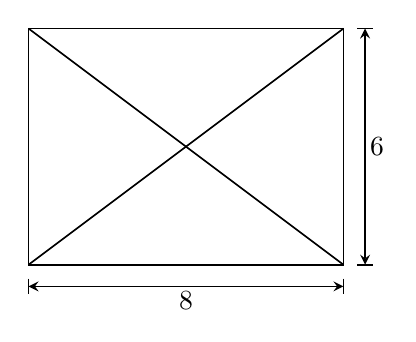
\begin{tikzpicture}[x=0.5cm, y=0.5cm, semithick,
  every node/.style={inner sep=1.5pt}]

  \draw (0,0) rectangle (8,6);
  \draw (0,0) -- (8,6);
  \draw (0,6) -- (8,0);

  % 下方尺寸线 8
  \draw[<->,>=stealth] (0,-0.55) -- (8,-0.55);
  \draw (0,-0.35) -- (0,-0.75);
  \draw (8,-0.35) -- (8,-0.75);
  \node[below] at (4,-0.55) {$8$};

  % 右侧尺寸线 6
  \draw[<->,>=stealth] (8.55,0) -- (8.55,6);
  \draw (8.35,0) -- (8.75,0);
  \draw (8.35,6) -- (8.75,6);
  \node[right] at (8.55,3) {$6$};
\end{tikzpicture}
\end{center}
\nopagebreak[4]
\Needspace{4\baselineskip}
\textbf{解析}

由三视图可知该几何体是四棱锥：底面为矩形，长 $8$、宽 $6$，高 $4$，顶点在底面中心正上方。

\Needspace{5\baselineskip}
（1）体积

\nopagebreak[4]
\[V=\frac13\times8\times6\times4=64.\]

\Needspace{5\baselineskip}
（2）前、后两个侧面的底边为 $8$，斜高为顶点到底面长边中点的距离：

\nopagebreak[4]
\[h_1=\sqrt{4^2+3^2}=5.\]

\Needspace{5\baselineskip}
左、右两个侧面的底边为 $6$，斜高为

\nopagebreak[4]
\[h_2=\sqrt{4^2+4^2}=4\sqrt2.\]

\Needspace{5\baselineskip}
故侧面积

\nopagebreak[4]
\[S=2\cdot\frac12\cdot8\cdot5+2\cdot\frac12\cdot6\cdot4\sqrt2=40+24\sqrt2.\]

（判断要点：斜高是顶点到底边的距离，不是棱长；两条斜高分别用底面半宽 $3$ 与半长 $4$ 计算。）

\gkanswer{答案：（1）$V=64$；（2）$S=40+24\sqrt2$。}

\end{answer}
\begin{answer}
\gksolhead{18}{}

\textbf{题目}：

下表提供了某厂节能降耗技术改造后生产甲产品过程中记录的产量 $x$（吨）与相应的生产能耗 $y$（吨标准煤）的几组对照数据。

\begin{center}
\begin{tabular}{lllll}
\toprule
$x$ & $3$ & $4$ & $5$ & $6$ \\
\midrule
$y$ & $2.5$ & $3$ & $4$ & $4.5$ \\
\bottomrule
\end{tabular}
\end{center}

（1）请画出上表数据的散点图；

（2）请根据上表提供的数据，用最小二乘法求出 $y$ 关于 $x$ 的线性回归方程 $\hat y=\hat b x+\hat a$；

（3）已知该厂技改前 $100$ 吨甲产品的生产能耗为 $90$ 吨标准煤。试根据（2）求出的线性回归方程，预测生产 $100$ 吨甲产品的生产能耗比技改前降低多少吨标准煤？

（参考数值：$3\times2.5+4\times3+5\times4+6\times4.5=66.5$）

\Needspace{4\baselineskip}
\textbf{解析}

（1）以 $x$ 为横轴、$y$ 为纵轴描出 $(3,2.5)$，$(4,3)$，$(5,4)$，$(6,4.5)$ 四点，散点大致沿一条上升直线分布。

\Needspace{5\baselineskip}
（2）$\bar x=\dfrac{3+4+5+6}{4}=4.5$，$\bar y=\dfrac{2.5+3+4+4.5}{4}=3.5$，且

\nopagebreak[4]
\[\sum_{i=1}^4x_iy_i=66.5,\qquad \sum_{i=1}^4x_i^2=9+16+25+36=86.\]

\Needspace{5\baselineskip}
于是

\nopagebreak[4]
\[\hat b=\frac{66.5-4\times4.5\times3.5}{86-4\times4.5^2}=\frac{3.5}{5}=0.7,\]

\nopagebreak[4]
\[\hat a=\bar y-\hat b\bar x=3.5-0.7\times4.5=0.35.\]

\Needspace{5\baselineskip}
故线性回归方程为

\nopagebreak[4]
\[\hat y=0.7x+0.35.\]

\Needspace{5\baselineskip}
（3）$x=100$ 时

\nopagebreak[4]
\[\hat y=0.7\times100+0.35=70.35.\]

\Needspace{5\baselineskip}
技改前为 $90$ 吨标准煤，故降低

\nopagebreak[4]
\[90-70.35=19.65\ \text{\text{吨标准煤}}.\]

（判断要点：回归系数公式中分子分母都用 $n\bar x\bar y$ 与 $n\bar x^2$ 修正；题给的参考数值 $66.5$ 直接用于分子。）

\gkanswer{答案：（2）$\hat y=0.7x+0.35$；（3）降低 $19.65$ 吨标准煤。}

\end{answer}
\begin{answer}
\gksolhead{19}{}

\textbf{题目}：

在平面直角坐标系 $xOy$ 中，已知圆心在第二象限，半径为 $2\sqrt2$ 的圆 $C$ 与直线 $y=x$ 相切于坐标原点 $O$。椭圆 $\dfrac{x^2}{a^2}+\dfrac{y^2}{9}=1$ 与圆 $C$ 的一个交点到椭圆两焦点的距离之和为 $10$。

（1）求圆 $C$ 的方程；

（2）试探究 $C$ 上是否存在异于原点的点 $Q$，使 $Q$ 到椭圆右焦点 $F$ 的距离等于线段 $OF$ 的长。若存在，请求出点 $Q$ 的坐标；若不存在，请说明理由。

\Needspace{4\baselineskip}
\textbf{解析}

\Needspace{5\baselineskip}
（1）圆与直线 $y=x$ 在原点相切，故圆心在过原点且垂直于 $y=x$ 的直线 $y=-x$ 上。设圆心为 $(-t,t)$（$t>0$），则半径

\nopagebreak[4]
\[r=\frac{|(-t)-t|}{\sqrt2}=\sqrt2t=2\sqrt2,\]

\Needspace{5\baselineskip}
得 $t=2$，圆心 $(-2,2)$，圆方程为

\nopagebreak[4]
\[(x+2)^2+(y-2)^2=8.\]

（2）椭圆上的点到两焦点距离之和为 $2a=10$，故 $a=5$；又 $b=3$，$c=\sqrt{a^2-b^2}=4$，右焦点 $F(4,0)$，$OF=4$。

\Needspace{5\baselineskip}
设 $Q(x,y)$，条件为

\nopagebreak[4]
\[(x+2)^2+(y-2)^2=8,\qquad (x-4)^2+y^2=16.\]

\Needspace{5\baselineskip}
两式相减：

\nopagebreak[4]
\[(x+2)^2-(x-4)^2+(y-2)^2-y^2=-8,\]

\Needspace{5\baselineskip}
即 $12x-4y-8=-8$，得 $y=3x$。代入第二式：

\nopagebreak[4]
\[(x-4)^2+9x^2=16,\qquad 10x^2-8x=0,\]

故 $x=0$（对应原点，题设要求异于原点，舍去）或 $x=\dfrac45$，$y=\dfrac{12}{5}$。检验：$\left(\dfrac45+2\right)^2+\left(\dfrac{12}{5}-2\right)^2=\dfrac{196}{25}+\dfrac{4}{25}=8$，在圆上。

故存在 $Q\left(\dfrac45,\dfrac{12}{5}\right)$。

（判断要点：相切条件是圆心到切线距离等于半径，且圆心在过切点的法线上；解出两组交点后必须用「异于原点」舍去一组。）

\gkanswer{答案：（1）$(x+2)^2+(y-2)^2=8$；（2）存在，$Q\left(\dfrac45,\dfrac{12}{5}\right)$。}

\end{answer}
\begin{answer}
\gksolhead{20}{}

\textbf{题目}：

已知函数 $f(x)=x^2+x-1$，$\alpha$，$\beta$ 是方程 $f(x)=0$ 的两个根（$\alpha>\beta$），$f'(x)$ 是 $f(x)$ 的导数，设 $a_1=1$，$a_{n+1}=a_n-\dfrac{f(a_n)}{f'(a_n)}$（$n=1,2,\cdots$）。

（1）求 $\alpha$，$\beta$ 的值；

（2）已知对任意的正整数 $n$，都有 $a_n>\alpha$，记 $b_n=\ln\dfrac{a_n-\beta}{a_n-\alpha}$（$n=1,2,\cdots$），求数列 $\{b_n\}$ 的前 $n$ 项和 $S_n$。

\Needspace{4\baselineskip}
\textbf{解析}

\Needspace{5\baselineskip}
（1）解 $x^2+x-1=0$：

\nopagebreak[4]
\[x=\frac{-1\pm\sqrt{1+4}}{2}=\frac{-1\pm\sqrt5}{2}.\]

\Needspace{5\baselineskip}
由 $\alpha>\beta$ 得

\nopagebreak[4]
\[\alpha=\frac{\sqrt5-1}{2},\qquad \beta=-\frac{\sqrt5+1}{2}.\]

\Needspace{5\baselineskip}
（2）由 $f(x)=(x-\alpha)(x-\beta)$ 及 $f'(x)=2x+1=(x-\alpha)+(x-\beta)$，

\nopagebreak[4]
\[a_{n+1}-\alpha=a_n-\alpha-\frac{(a_n-\alpha)(a_n-\beta)}{(a_n-\alpha)+(a_n-\beta)}=\frac{(a_n-\alpha)^2}{(a_n-\alpha)+(a_n-\beta)},\]

\Needspace{5\baselineskip}
同理

\nopagebreak[4]
\[a_{n+1}-\beta=\frac{(a_n-\beta)^2}{(a_n-\alpha)+(a_n-\beta)}.\]

\Needspace{5\baselineskip}
相除得

\nopagebreak[4]
\[\frac{a_{n+1}-\beta}{a_{n+1}-\alpha}=\left(\frac{a_n-\beta}{a_n-\alpha}\right)^2,\]

即 $b_{n+1}=2b_n$，故 $\{b_n\}$ 是公比为 $2$ 的等比数列。

\Needspace{5\baselineskip}
计算首项：$a_1=1$，

\nopagebreak[4]
\[\frac{1-\beta}{1-\alpha}=\frac{1+\frac{\sqrt5+1}{2}}{1-\frac{\sqrt5-1}{2}}=\frac{3+\sqrt5}{3-\sqrt5}=\frac{(3+\sqrt5)^2}{4}=\frac{7+3\sqrt5}{2}.\]

\Needspace{5\baselineskip}
令 $\varphi=\dfrac{1+\sqrt5}{2}$，则 $\varphi^2=\dfrac{3+\sqrt5}{2}$，$\dfrac{7+3\sqrt5}{2}=\varphi^4$，故

\nopagebreak[4]
\[b_1=\ln\varphi^4=4\ln\varphi=2\ln\frac{3+\sqrt5}{2}.\]

\Needspace{5\baselineskip}
于是

\nopagebreak[4]
\[S_n=\frac{b_1(1-2^n)}{1-2}=2(2^n-1)\ln\frac{3+\sqrt5}{2}.\]

（判断要点：牛顿迭代式的关键是利用 $\alpha,\beta$ 是因式分解出平方结构，再相除得等比；首项要化简成 $\varphi$ 的幂，否则 $S_n$ 形式不整洁。）

\gkanswer{答案：（1）$\alpha=\dfrac{\sqrt5-1}{2}$，$\beta=-\dfrac{\sqrt5+1}{2}$；（2）$S_n=2(2^n-1)\ln\dfrac{3+\sqrt5}{2}$。}

\end{answer}
\begin{answer}
\gksolhead{21}{}

\textbf{题目}：

已知 $a$ 是实数，函数 $f(x)=2ax^2+2x-3-a$。如果函数 $y=f(x)$ 在区间 $[-1,1]$ 上有零点，求 $a$ 的取值范围。

\Needspace{4\baselineskip}
\textbf{解析}

$a=0$ 时 $f(x)=2x-3$，零点 $x=\dfrac32\notin[-1,1]$，不合题意。

\Needspace{5\baselineskip}
$a\neq0$ 时，$f(x)=0$ 等价于

\nopagebreak[4]
\[a(2x^2-1)=3-2x,\qquad a=\frac{3-2x}{2x^2-1}=:g(x),\]

\Needspace{5\baselineskip}
定义域为 $x\in[-1,1]$ 且 $x\neq\pm\dfrac{\sqrt2}{2}$。

\nopagebreak[4]
\[g'(x)=\frac{-2(2x^2-1)-(3-2x)\cdot4x}{(2x^2-1)^2}=\frac{4x^2-12x+2}{(2x^2-1)^2}=\frac{2(2x^2-6x+1)}{(2x^2-1)^2}.\]

驻点为 $x=\dfrac{3\pm\sqrt7}{2}$，其中只有 $x_0=\dfrac{3-\sqrt7}{2}\in(-1,1)$。

分段考察：

$\left[-1,-\dfrac{\sqrt2}{2}\right)$ 上 $g$ 单调递增，$g(-1)=5$，$x\to-\dfrac{\sqrt2}{2}^-$ 时 $g\to+\infty$，值域 $[5,+\infty)$；

\Needspace{5\baselineskip}
$\left(-\dfrac{\sqrt2}{2},\dfrac{\sqrt2}{2}\right)$ 上 $g$ 从 $-\infty$ 增到极大值再减到 $-\infty$，极大值为

\nopagebreak[4]
\[g\left(\frac{3-\sqrt7}{2}\right)=-\frac{3+\sqrt7}{2},\]

值域 $\left(-\infty,-\dfrac{3+\sqrt7}{2}\right]$；

$\left(\dfrac{\sqrt2}{2},1\right]$ 上 $g$ 从 $+\infty$ 单调递减到 $g(1)=1$，值域 $[1,+\infty)$。

\Needspace{5\baselineskip}
综上，$a$ 的取值范围是

\nopagebreak[4]
\[\left(-\infty,-\frac{3+\sqrt7}{2}\right]\cup[1,+\infty).\]

（判断要点：分离参数后要按 $2x^2-1$ 的符号分段，渐近线 $x=\pm\dfrac{\sqrt2}{2}$ 两侧值域方向相反；$g(-1)=5$ 落在 $[1,+\infty)$ 内，不会产生新的端点。）

\gkanswer{答案：$a\leqslant-\dfrac{3+\sqrt7}{2}$ 或 $a\geqslant1$。}

\end{answer}